\section{Fahrspurregelung mittels modellprädiktiver Regelung}
In allen dynamischen Disziplienen des Carolocups besteht die wichtige Teilaufgabe möglichst fehlerfrei einer aufgeklebten Fahrspur zu folgen. Um diese Aufgabe zu erfüllen, wurde ein modellprädiktiver Regelansatz gewählt.\\ \\ 
Bei der modellprädiktiven Regelung (MPC) handelt es sich um eine Form der optimalen Regelung, bei der wiederholt eine Berechnung der optimalen Steuerung für ein System ausgehend von dessen aktuellem Zustand stattfindet. In vielen Bereichen finden MPCs immer häufiger Anwendung, da sie eine direkte Berücksichtigung von Beschränkungen erlauben und eine Form des strukturierten Reglerentwurfs ausgehend von der modellierten Systemdynamik darstellen. Dabei kann durch die geeignete Wahl der Kostenfunktion und deren Wichtungsparametern die Güte der des Reglers geziehlt beeinflusst werden. Allerdings ergeben sich auch Schwierigkeiten bei der Verwendung von MPCs. Zum einen ist die Konvergenz der Optimierung gegen einen optimalen Wert für die Optimierungsvariablen und die Stabiltät des geschlossenen Kreises insbesondere bei nichtlinearen Systemmodellen oft nur schwierig nachweisbar und zum anderen stellt das wiederholte Lösen des meist hochdimensionalen Optimierungsproblems während der Laufzeit in genügend schneller Geschwindigkeit eine große Herausforderung dar.
\\
\subsection{Problemformulierung für die modellprädiktive Regelung}
Im realen Anwenungsfall des oTToCAR-Projekts eignet sich eine Systemdarstellung in zeitdiskreter Form, bei der die Lösung des Optimierungsproblems weniger komplex ist und die ebenfalls zeitdiskreten Messwerte vom realen System weniger kompliziert integriert werden können. Demnach sind die diskretisierten Systemgleichungen wiefolgt gegeben:
\begin{align*}
  \boldsymbol{x}(k+1)&=\boldsymbol{f}\left ( \boldsymbol{x}(k), \boldsymbol{u}(k) \right )\\
  \boldsymbol{y}(k)&=\boldsymbol{g}\left ( \boldsymbol{x}(k) \right )\\
\end{align*}
mit den nichtlinearen Funktionen $\boldsymbol{f}\left ( \cdot \right )$ und $\boldsymbol{g}\left ( \cdot \right )$, wobei
\begin{align*}
  &\boldsymbol{x}(k) \in \mathcal{X}\subset\mathbb{R}^n\\
  &\boldsymbol{u}(k) \in \mathcal{U}\subset\mathbb{R}^m\\
  &\boldsymbol{y}(k) \in \mathcal{Y}\subset\mathbb{R}^r
\end{align*}
Ausgehend vom aktuellen Zustand $\boldsymbol{x}(k)$ des zu regelnden Systems, der wenn nicht messbar geschätzt werden muss, wird anhand des Systemmodells das zukünftige Systemverhalten
\begin{align*}
  \boldsymbol{x_p}=\left\{ \boldsymbol{x}(k+1),\dots,\boldsymbol{x}(k+n_p)\right\}
\end{align*}
bis zum Prädiktionshorizont $n_p$ unter der Optimierung einer Sequenz von Eingängen
\begin{align*}
  \boldsymbol{u}=\left\{ \boldsymbol{u}(k),\dots,\boldsymbol{u}(k+n_c-1)\right\}
\end{align*}
bis zum Stellhorizont $n_c$ vorhergesagt. Aus der gefundenen optimalen Eingangssequenz $\boldsymbol{u}^*$ wird der erste Eintrag $\boldsymbol{u}^*(k)$ auf das zu regelnde System angewandt. Im nächsten Zeitschritt kann der neue Zustand gemessen bzw. geschätzt werden und die Optimierung beginnt von neuem. Ziel dabei ist es einer Referenztrajektorie $\boldsymbol{x_r}$ zu folgen.\\ \\
Für das an jedem Zeitschritt $k$ zu lösende Minimierungsproblem wurde die benötigte Kostenfunktion $J$ in quadratische Form mit $\boldsymbol{x_p}$ und $\boldsymbol{u}$ als Optimierungsvariablen aufgestellt:
\begin{align*}
	\underset{\boldsymbol{x_p, u}}{\text{min}}\;&J:=\sum_{i=k+1}^{k+n_p} \left [\boldsymbol{x}_{p}(i)-\boldsymbol{x}_{r}(i)\right ]^T\boldsymbol{Q}_i\left [\boldsymbol{x}_{p}(i)-\boldsymbol{x}_{r}(i)\right ] +\sum_{j=k}^{k+n_c-1} \boldsymbol{u}^T(j)\boldsymbol{R}_j\boldsymbol{u}(j)\\
	s.t.\;&\boldsymbol{x_p}(i+1)=\boldsymbol{f}\left ( \boldsymbol{x_p}(i), \boldsymbol{u}(i) \right ),\quad i=k,...,k+n_c-1\\
	&\boldsymbol{x_p}(i+1)=\boldsymbol{f}\left ( \boldsymbol{x_p}(i), \boldsymbol{u}(k+n_c-1) \right ),\quad i=k+n_c,...,k+n_p-1
\end{align*}
Mit den Vektoren
\begin{align*}
	\boldsymbol{x}_p(k)&=\left [ \boldsymbol{x}_p(k+1\mid k),\dots,\boldsymbol{x}_p(k+n_p\mid k) \right ]^T\\
	\boldsymbol{x}_r(k)&=\left [ \boldsymbol{x}_r(k+1),\dots,\boldsymbol{x}_r(k+n_p) \right ]^T\\
	\boldsymbol{u}(k)&=\left [ \boldsymbol{u}(k),\dots,\boldsymbol{u}(k+n_c-1) \right ]^T
\end{align*}
und dazugehörigen Wichtungsmatrizen $\boldsymbol{Q}_i\;(i=1, ...,n_p)$ und $\boldsymbol{R}_j\;(j=0, ...,n_c-1)$, die folgende Vorausetzungen erfüllen müssen.\\
Linear MPC/Nonlinear MPC\\
Beschränkungen
\subsection{Konkrete Implementierung der Fahrspurregelung für das oTToCAR}
Die konkrete Implementierung der Fahrspurregelung auf der Recheneinheit des oTToCARs macht weitere Vorabeit, wie das erstellen der Referenztrajektorie und Anpassungen des allgemeinen Anstatzes für die MPC wie gewisse Vereinfachungen, um die Regelung mit einer Rate von 50Hz betreiben zu können, nötig.
\subsubsection{Dimension der Optimierungsvariable}
Als Systemeingänge für das Fahrzeugmodell sind eine abstrakte Entsprechung des Motordrehmoments $u_1=...$ und der Lenkeinschlag der Räder $u_2=...$ vorhanden, demnach ergibt sich der Stellgrößenvektor zum Zeitpunkt $k$ zu $\boldsymbol{u}(k)=[u_1(k), u_2(k)]^T$. Da sich die prädizierten Zustände $\boldsymbol{x}_p$ aus den Gleichungsnebenbedingungen berechnen lassen, ergibt sich die Diemension der Optimierungsvariable also zu $2\cdot n_c$.
Je größer man $n_c$ wählt, desto besser lässt sich z.B. die Geschwindigkeit in Abhängigkeit zur Entfernung und Krümmung einer bevorstehenden Kurve begrenzen oder Schwierigkeiten beim Durchfahren von S-Kurven bewältigen. Allerdings nimmt dadurch auch die Dimension der Optimierungsvariable zu, was dazu führt, dass die Grenzen der verfügbaren Rechenzeit zum Lösen des Optimierungsproblems während der Laufzeit schnell erreicht werden.
\subsubsection{Referenztrajektorie}
Mit einer auf dem Fahrzeug befestigten Kamera lässt sich die zu verfolgende Fahrbahn wahrnehmen. Diese Wahrnehmung liefert mit einer Rate von bis zu 50Hz eine Polylinie der erkannten Fahrbahnmarkierung projeziert auf die rechte Fahrspur. Diese Polyline kann je nach erkannter Fahrbahn aus einer unterschiedlich Anzahl von Punkten mit variablem Abstand zu einander bestehen.\\ \\
Um diese Polylinien als Referenztrajektorie für die MPC nutzen zu können, werden zu kurze Polylinien zunächst soweit extrapoliert, dass ein Vergleich zwischen Prädiktion zum Zeitschritt $k+np$ und Referenz in jedem Fall möglich ist. Anschließend werden die Koordinaten der Punkte auf der Polylinie als Funkion in Abhängigkeit der summierten Wegstrecke zwischen den Punkten vom Auto ausgehend hinterlegt, um diese dann als Referenztrajektorie zu jeder beliebigen Wegstrecke s = v*t*i interpolieren zu können.\\ \\
Kostenfunktion angepasst $x_p(i)-x_r((i-k)\Delta t)$
Das Modell liefert als $x_1$ und $x_2$ die Position des Autos auf einer globalen Karte und den Gierwinkel dazu. Da bisher noch keine globale Karte implementiert ist, wird jedes Mal, wenn eine neue Polylinie vorhanden ist die Pseudo-Weltkarte auf das Vehicle Reference Frame zurück gesetzt (Fahrzeugposition und Gierwinkel auf 0 setzen.) Es ist dann kurzeitig möglich, wenn keine neue Polylinie vorhanden ist, weiter an der letzten Referenztrajektorie weiter zu fahren, in dem man x(k) mit Hife des Modells schätzt.\\ \\
Referenz visualisieren: Plot der Punkte der Polylinie mit eingetragener Prädiktion des optimalen Lenkeinschlags\\
\begin{figure}[t]
\centering
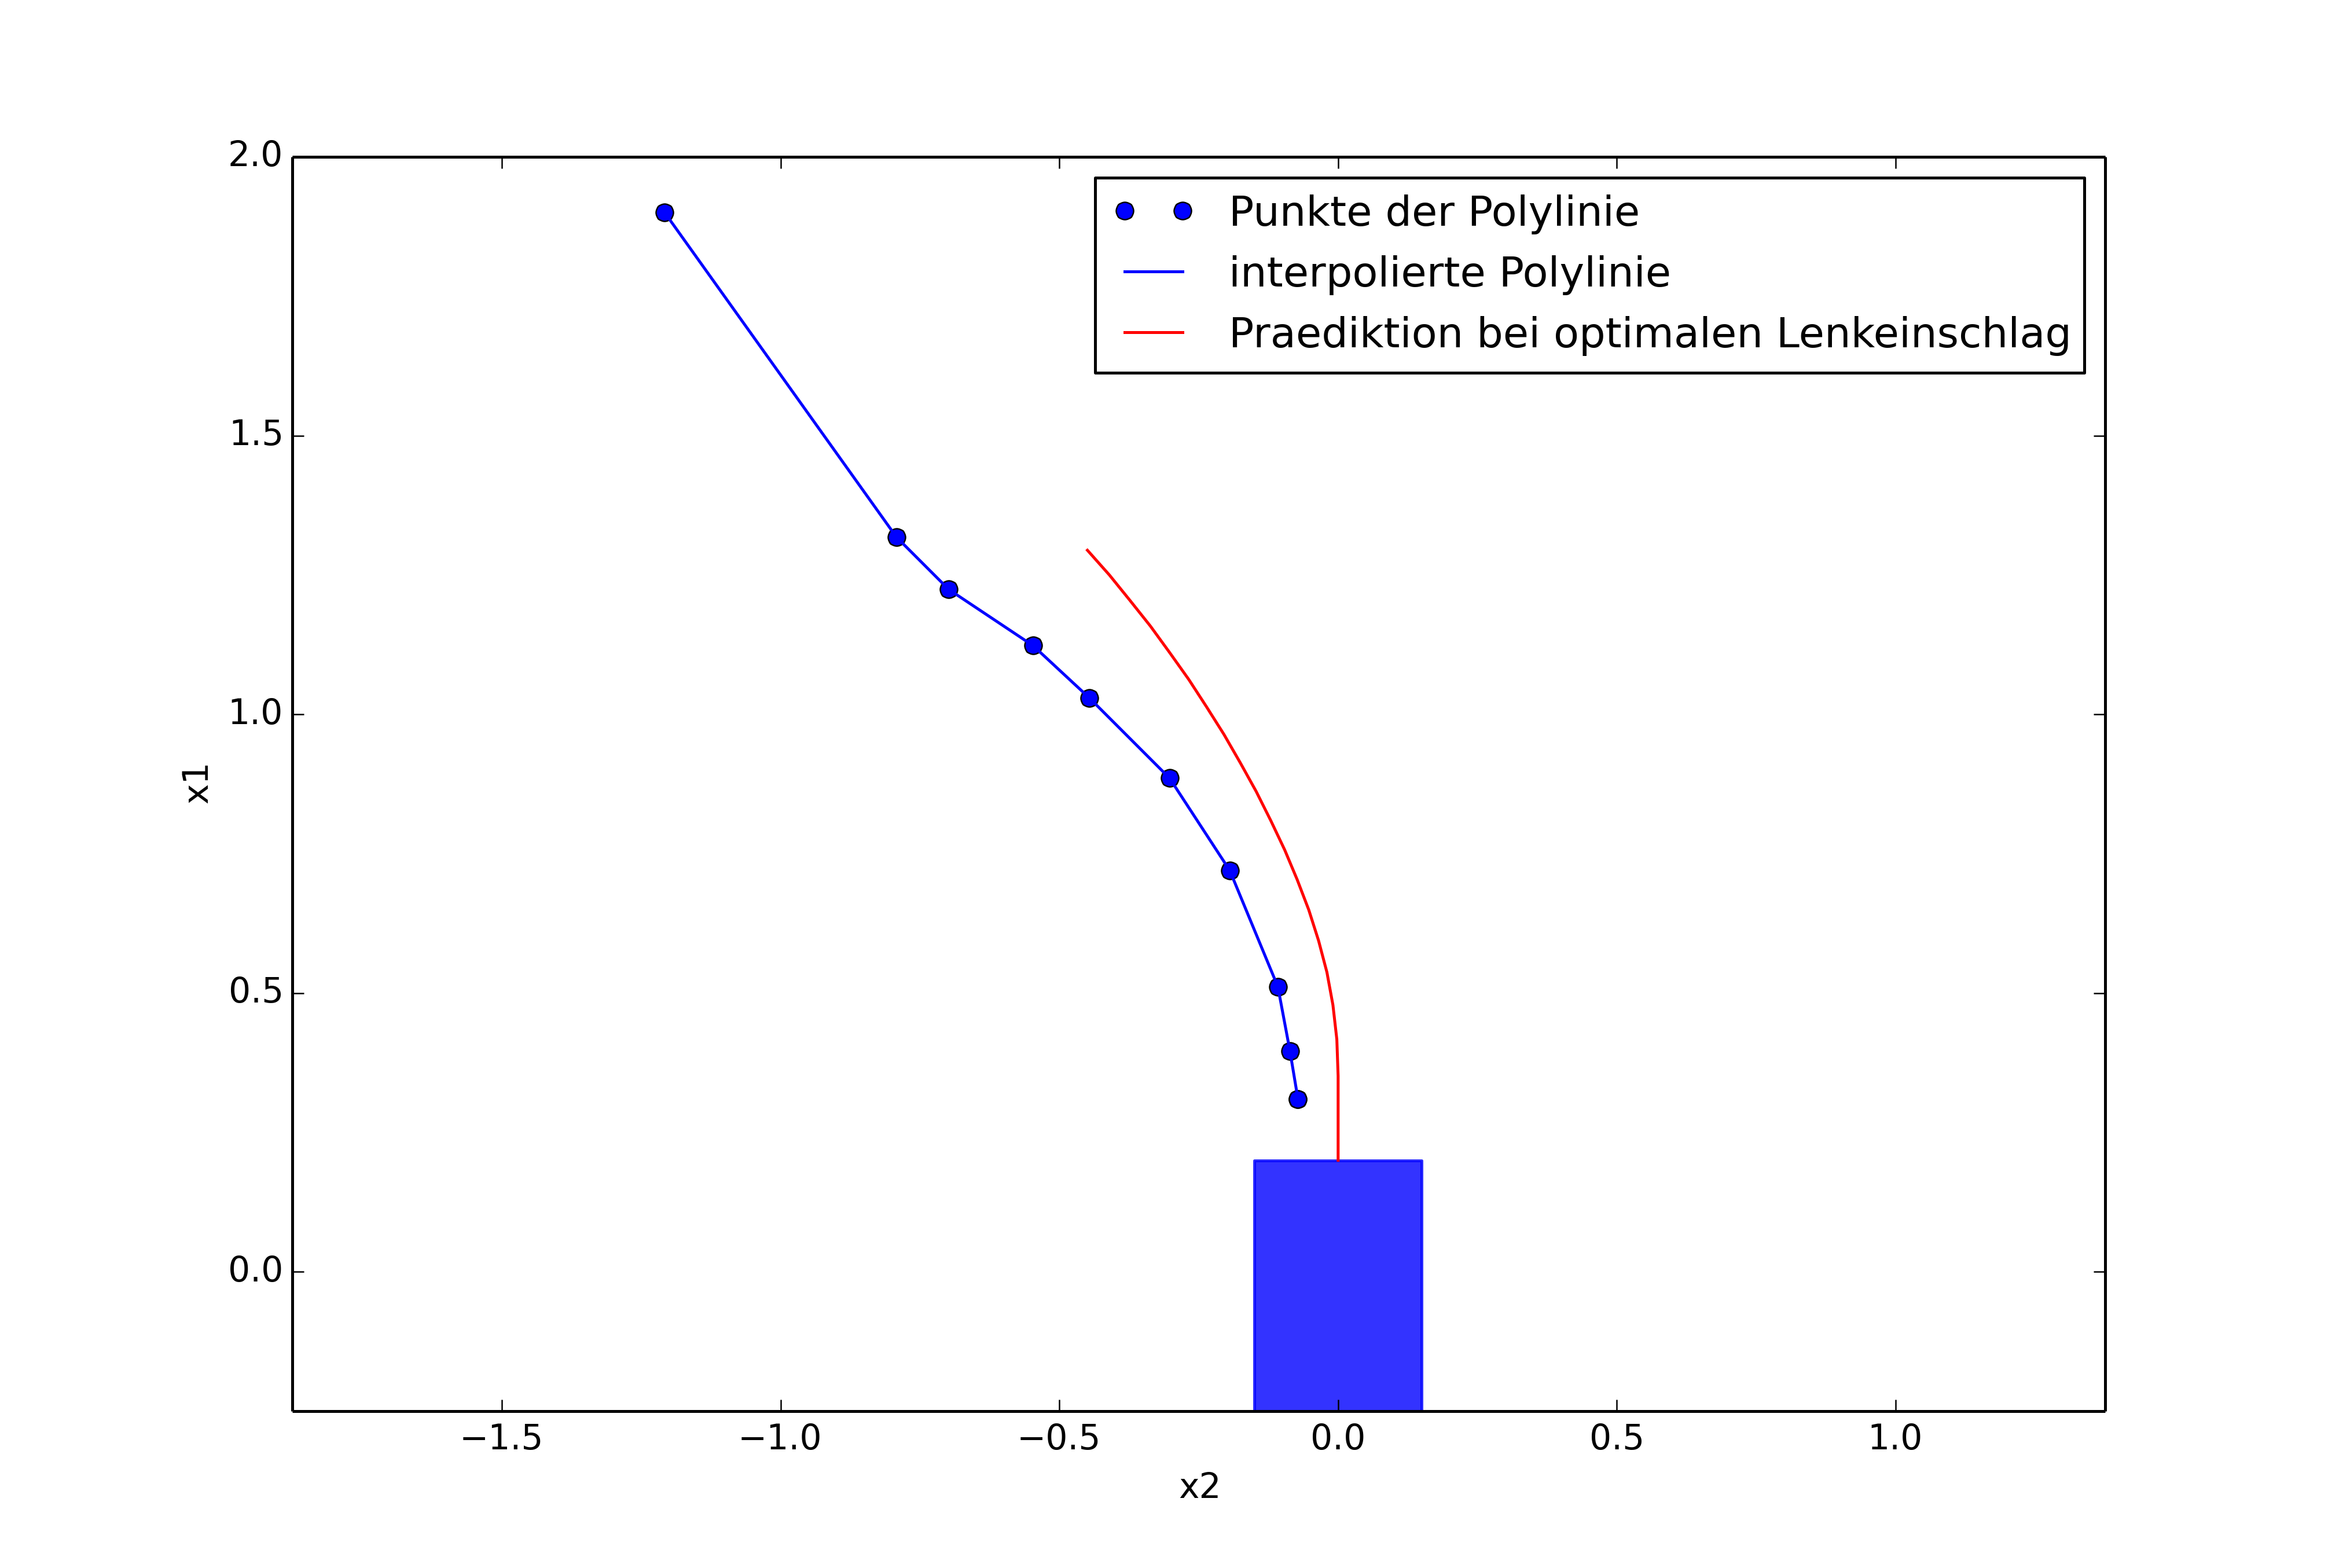
\includegraphics[scale=0.53]{Bilder/Reference.png}
\caption{Veranschaulichung der Referenztrajektorie und des prädizierten Verhaltens}
\end{figure}
\subsubsection{Vereinfachungen}
Aktuell wird die Motorsteuergröße nicht mitoptimiert und der Prädiktionshorizont beträgt 1. In dieser Konfiguration gibt es sicher Algorithmen wie LQR die Äquivalente Lösungen liefern und dabei besser nachweisbare Stabilität aufweisen. Es wurde sich trotzdem für die vereinfachte Variante entschieden, um diese in Zukunft so wie geplant zu erweitern.\\ \\
Es genügt den Scheitelpunkt der approximierten Variablen zu berechnen. genau genug.\\
Kostenfunktion wie Parabel im Bereich unseres Interesses, an kann mit 3 Funktionsaufrufen den Schritt bestimmen, der zum Approximierten Optimum führt. Durch genügend hohe Wiederholrate ist das Ergebnis genau genug.
Skalierbarkeit\\
Scheitelpunkt -> Newtonschritt der quadratischen Kostenfunktion\\

Lösen der Modellgleichungen mit konster geringer Geschwindigkeit, da für hohe Geschwindigkeiten noch keine passenden Modellparameter bestimmt werden konnten.
\subsubsection{Stabilität}
Um Sicher zu gehen, dass der Algorithmus immer gegen ein Optimum konvergiert wurde die in implementierten Fall skalare Kostenfunktionen in der Parcour fahrt in möglichst vielen denkbaren Positionen aufgenommen und überprüft, dass sich kein Fall ergibt, in dem das Optimierungsproblem in relevanten Bereich nicht convex ist.
\\
\\
\begin{figure}[t]
\centering
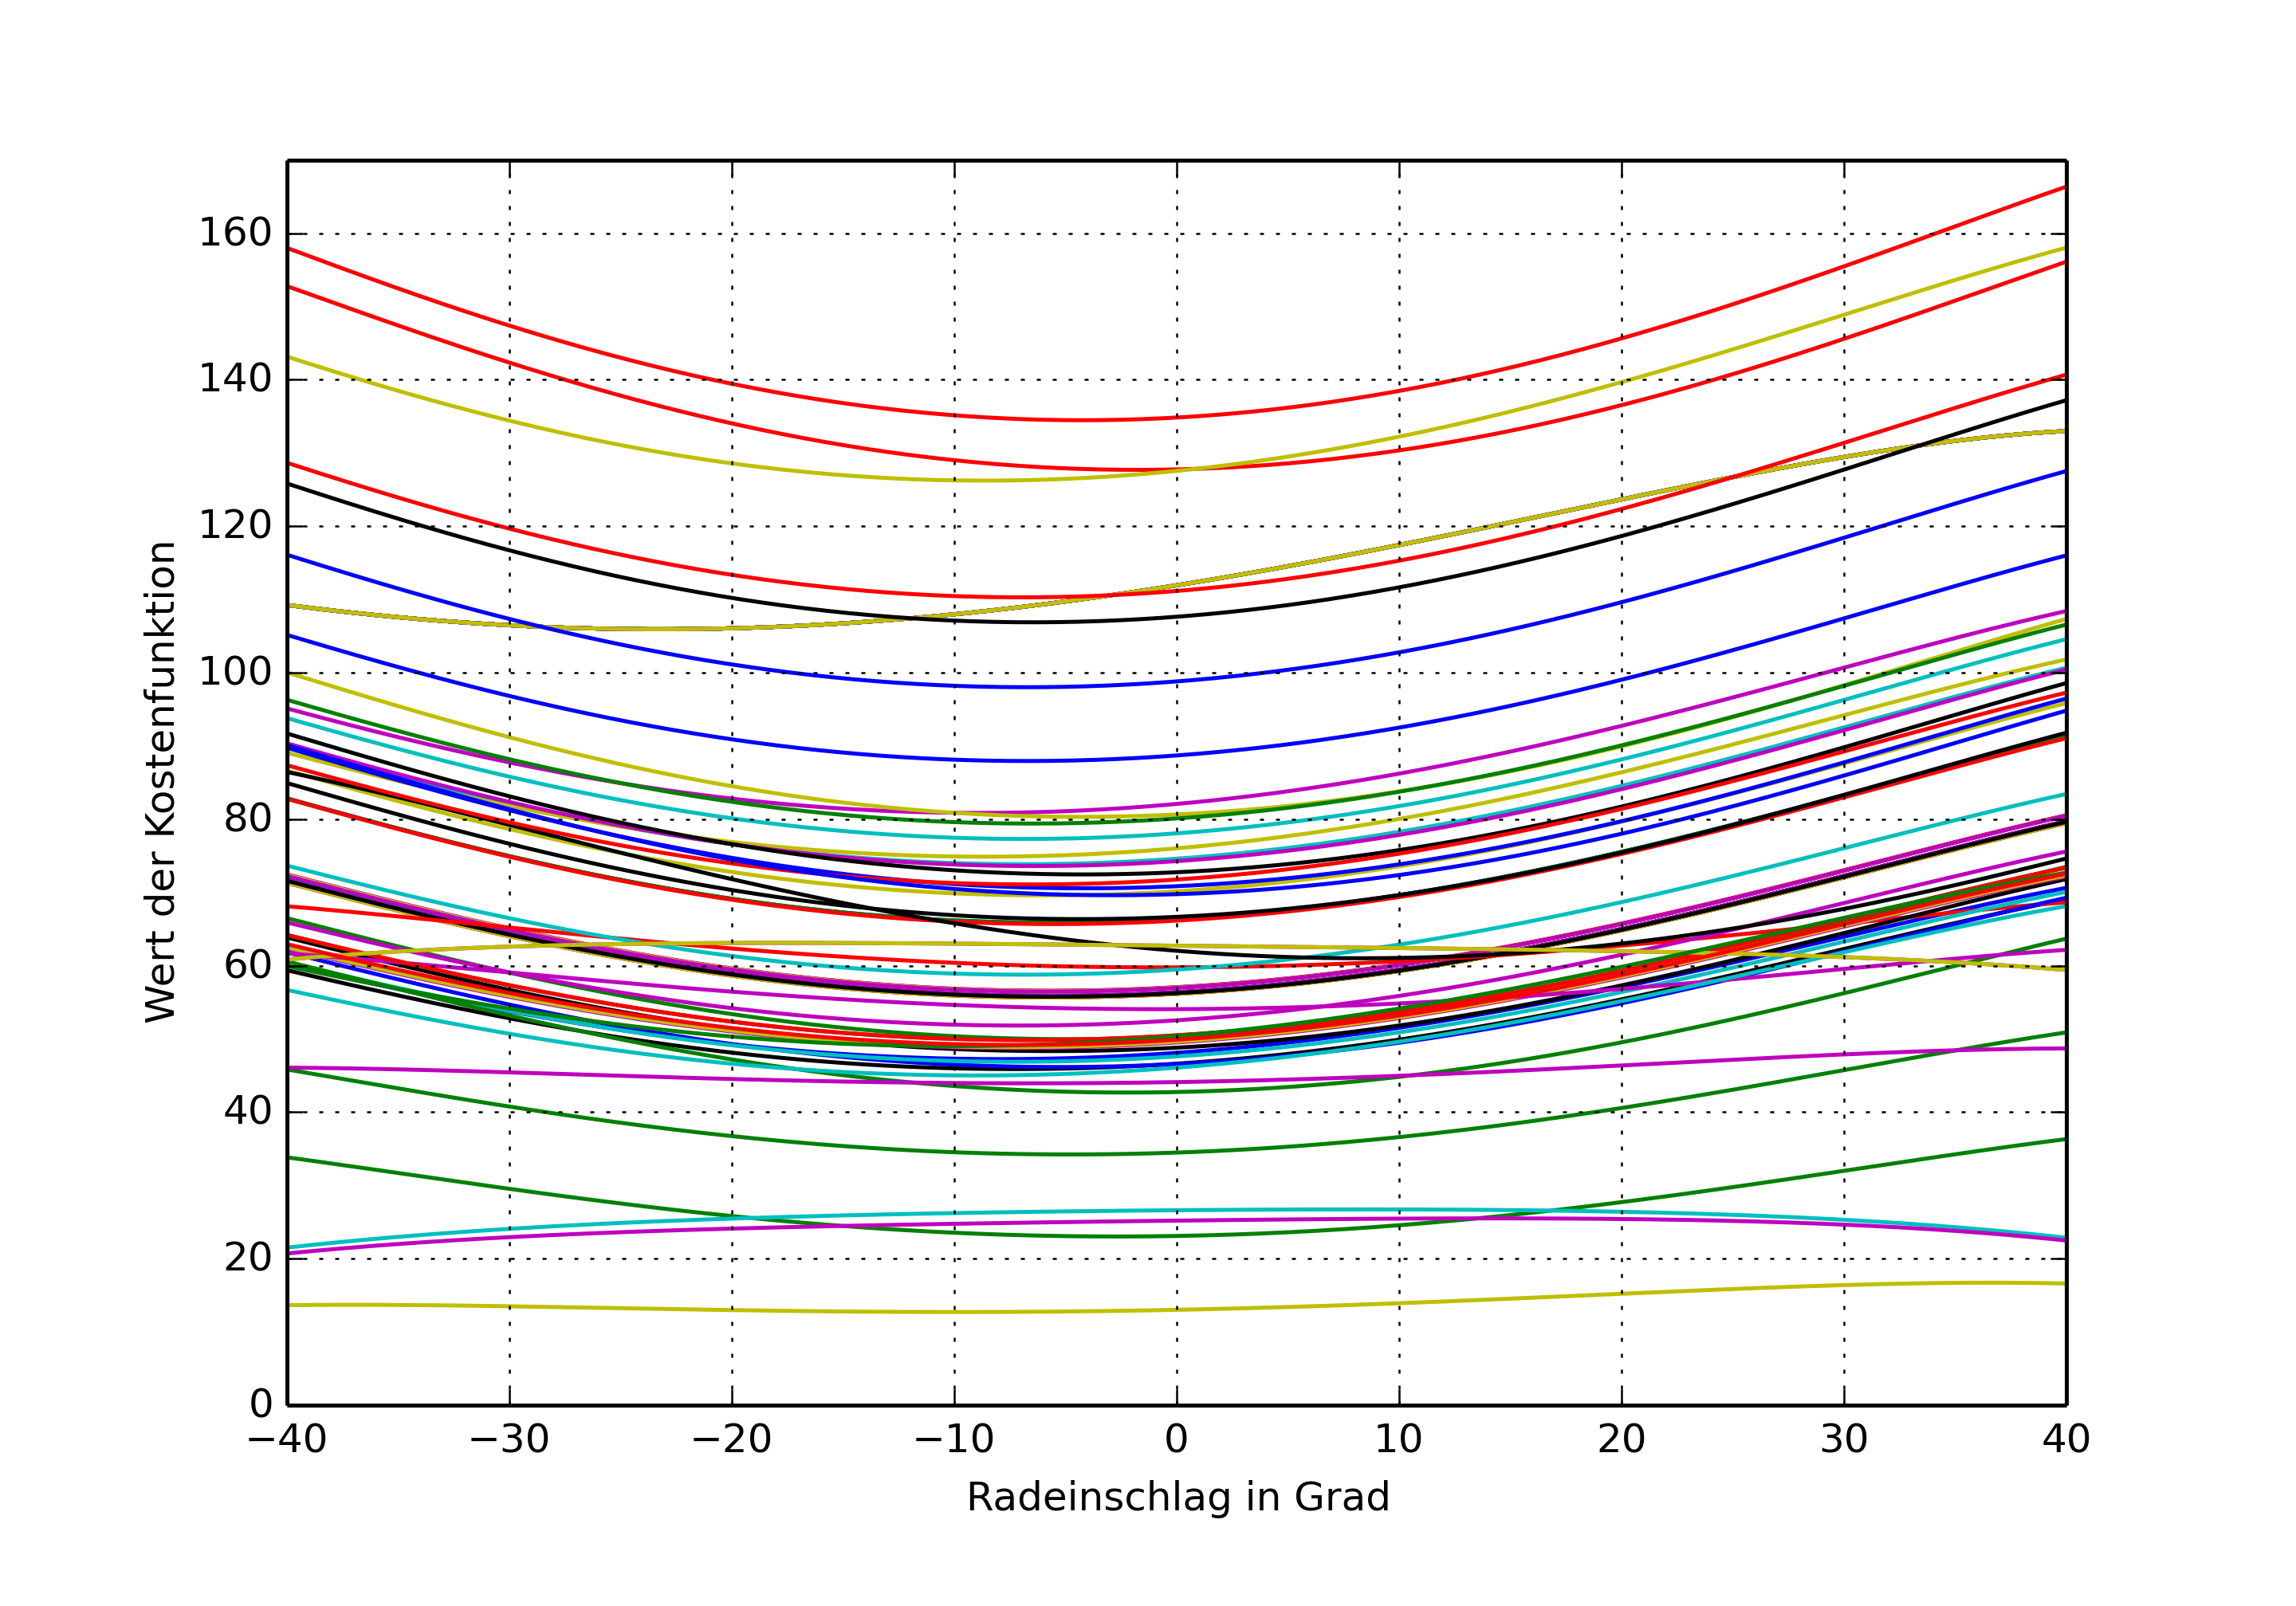
\includegraphics[scale=0.75]{Bilder/Parabeln.png}
\caption{Kostenfunktion in Abhängigkeit vom Radeinschlag in verschiedenen Fahrzeugpositionen}
\end{figure}

Aufwand\\
Nochmal überlegen\\

\subsubsection{Beschränkungen}
Hinzufügen von ~
\subsection{Spurwechsel}
Polylinie um Fahrspurbreite verschieben, wenn Hindernis erkannt. MPC findet optimale Trajektorie zu den verschobenen Punkten. Problem: Fahrspur verschwindet aus Sichtfeld. Langsameres Dosierteres Spurwechseln ist keine Lösung, da Hindernisse nach einer Kurve oft erst spät erkannt werden und deshalb Spurwechsel auf kurzer Distanz nötig sind. Lösung: Orientierung auf Karte

\subsection{Dynamic Reconfigure}
In der Vorbereitung auf den Wettkampf hat sich herausgestellt, dass die kurzen Testzeiten auf der Originalstrecke gut ausgenutzt werden muss. Dazu musste vorher extrahiert werden, welche Parameter entscheidenen Einfluss auf die Güte haben. Diese konnten dann online während der Fahrt mit dem dynamic reconfigure Paket getuned werden. (welche Parameter)\\
\subsection{Zukünftige Schritte}
Geschwindigkeit, mehrere Schritte in die Zukunft, Erstellung einer Karte mit Gewichtung der Confidence der Polylinien